\chapter{Introduction}
\label{chp:introduction}

Development of complex systems requires an efficient way for engineers to ensure the correctness of the developed software. \acrlong{dsm} (\acrshort{dsm}) can achieve this through automatic code generation and block-diagram visualizations, significantly reducing the risk of faulty applications and enabeling engineers to work more effectively.\\
In safety-critical development processes however, \acrshort{dsm} can only be used without subsequent manual verification, if the \acrshort{dsm} tools work correctly. This can either be achieved through time intensive qualified software development processes, which ensure accurate and reliable visualization of \acrshort{dsm} through the tool itself, or through the use of unverified \acrshort{dsm} tools followed by the subsequent use of a small visualization verification tool to ensure the correctness of the application.\\
In low-cost projects with high safety requirements, a cost-effective qualification method is crucial, highlighting the potential of the latter approach for a qualifiable graphical verification tool for use in \acrshort{dsm}.

The Institute for Aircraft Systems is currently developing a way for avionic models to be developed inside a web-based graphical model editor called \textit{\acrlong{xgee}} or \textit{\acrshort{xgee}}.\\
\acrshort{xgee} uses three kinds of \textit{tokens} within three distinct editors to visualize avionic models. They are:
\begin{itemize}
    \item signals
    \item vertices
    \item text labels
\end{itemize}
In \textit{\acrshort{xgee}}, each of the three editor models utilizes a unique set of \textit{.svg} files to represent different components within the avionic model. These editor models are the \textit{functions editor}, the \textit{hardware editor}, and the \textit{allocations editor}. An overview of these editors is provided in \autoref{fig:editors}.\\
The functions editor is used to define avionic functions and their interactions. Functions are represented as large blue boxes, with their interactions shown through black signals connecting inputs and outputs. Inputs and outputs are depicted as small black-and-white triangles located on the left and right edges of the function boxes. Inputs, outputs and functions have visible text labels.\\
The hardware editor is used to define hardware components and their physical connections. Hardware components are represented as large gray boxes, and their connections are illustrated by black signals linking \acrlong{io} (\acrshort{io}) ports. These \acrshort{io} ports appear as small black squares positioned along any edge of the hardware boxes. Like in the functions editor, \acrshort{io}s and devices have visible text labels.\\
The allocations editor is used to map functions to hardware components. In this editor, functions are represented as small blue boxes nested within larger gray hardware boxes. The specific signal transmissions between the hardware components are illustrated as white signal boxes that overlap with the corresponding physical connections. These boxes contain the signals being transmitted through the corresponding connection. Inside the gray hardware boxes, connections between functions and \acrshort{io}'s, are illustrated as thin, color-coded signals. However, these connections are purely visual within the allocations editor and do not contribute to the overall model structure.

This paper builds upon the work of \cite{waldvogel_annighoefer_models_2024} to further automate the verification process within \acrshort{xgee} by tokenizing a screenshot from within the editor. This means detecting the bounding boxes and token types of all elements of the diagram. To recognize and process the screenshot data, methods from the \textit{\acrshort{opencv}} Python library are being used.

\begin{figure}[h]
    \centering
    % First image
    \begin{subfigure}{0.3\textwidth}
        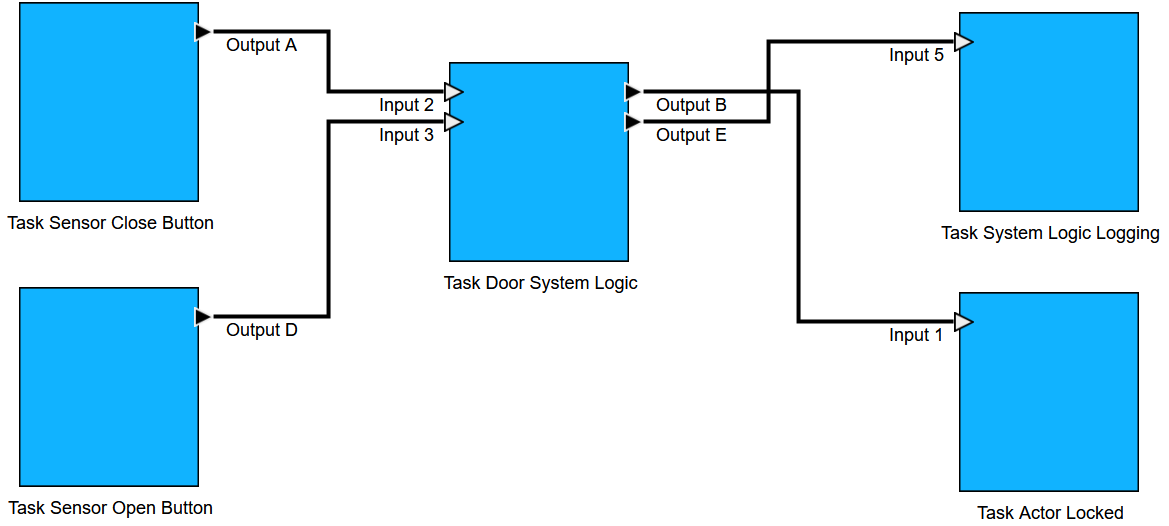
\includegraphics[width=\linewidth]{pictures/functions_editor.png}
        \caption{Functions editor}
        \label{fig:functions_editor}
    \end{subfigure}
    \hfill
    % Second image
    \begin{subfigure}{0.3\textwidth}
        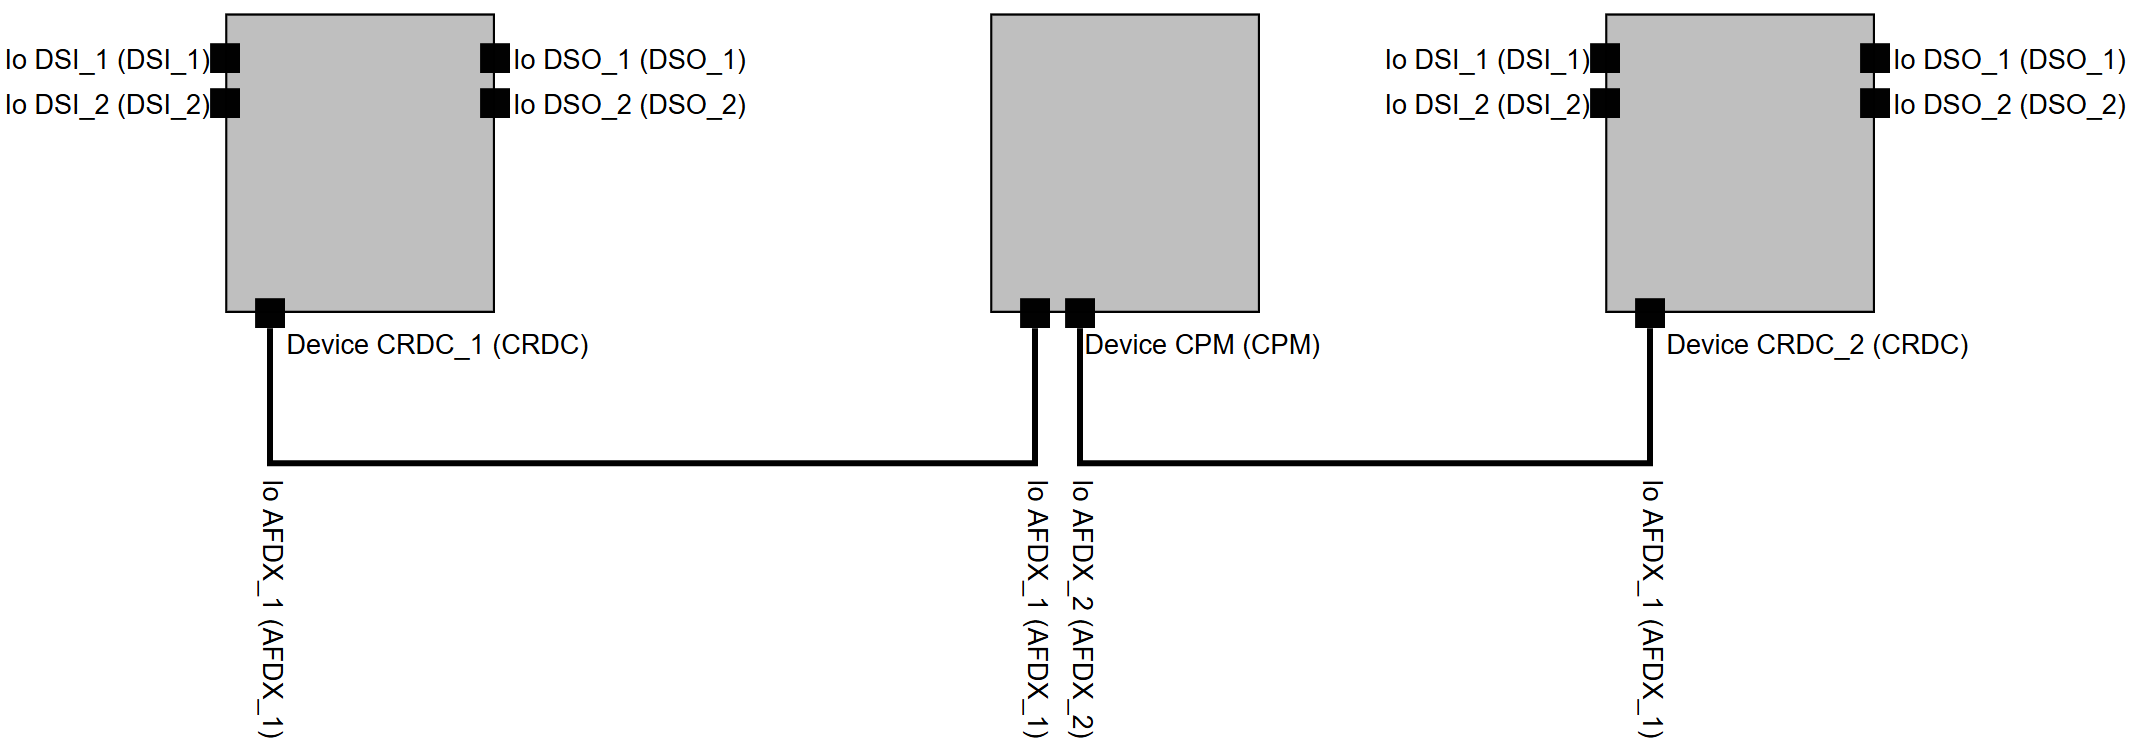
\includegraphics[width=\linewidth]{pictures/hardware_editor.png}
        \caption{Hardware editor}
        \label{fig:hardware_editor}
    \end{subfigure}
    \hfill
    % Third image
    \begin{subfigure}{0.3\textwidth}
        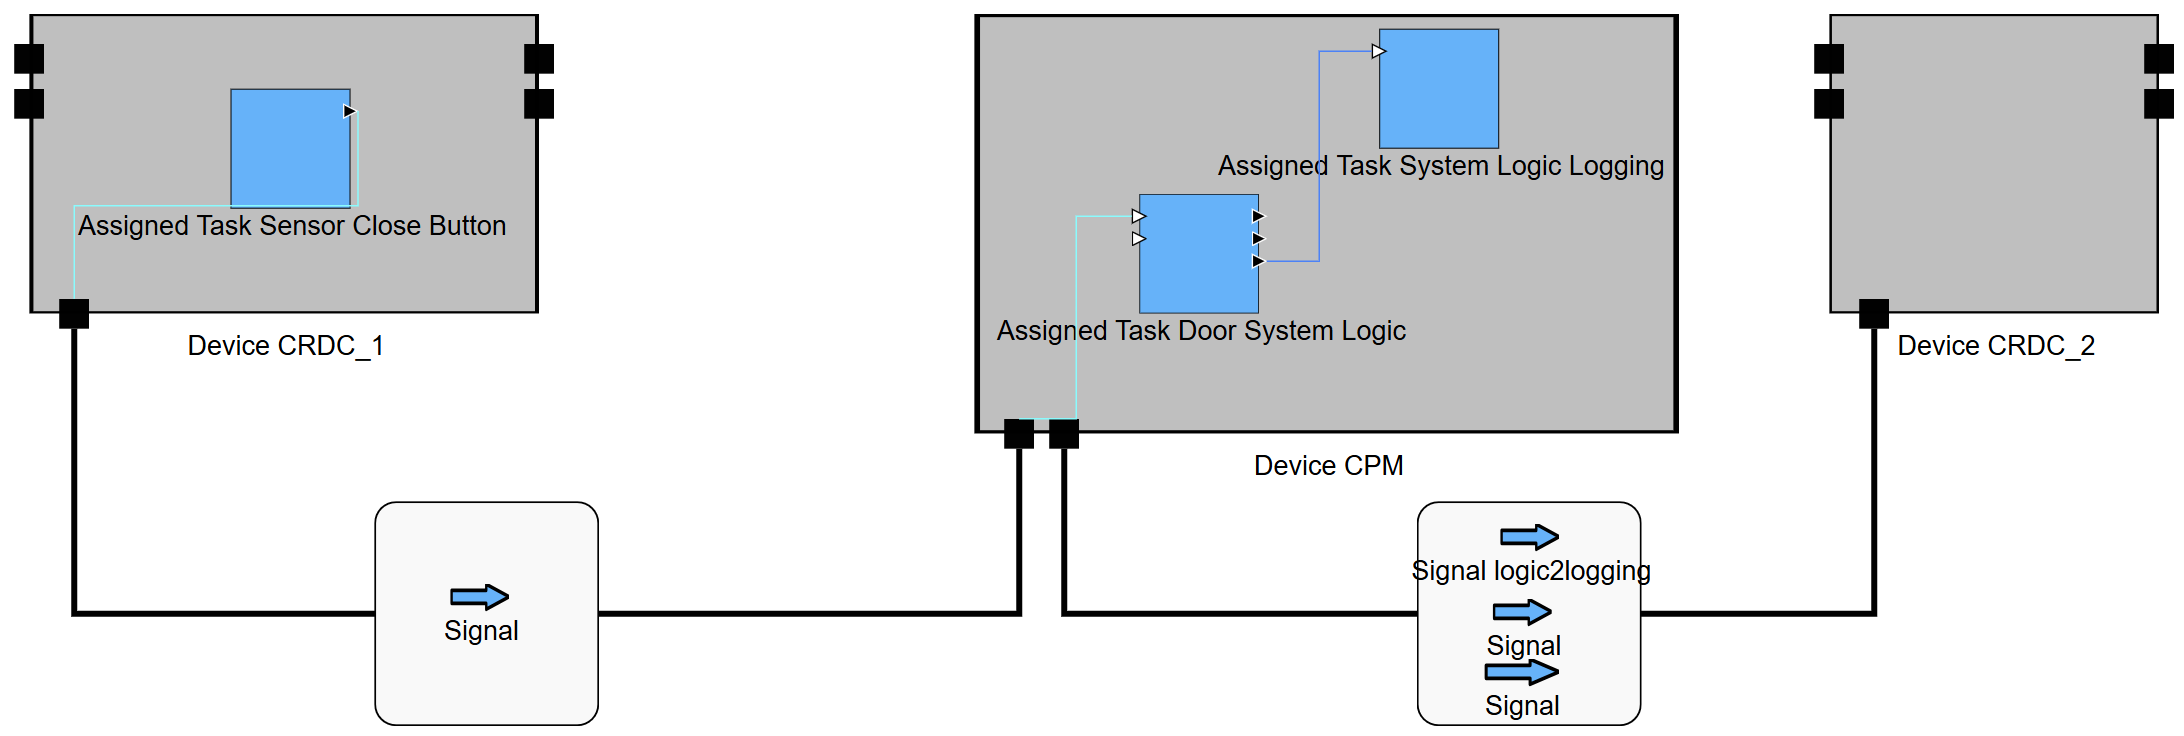
\includegraphics[width=\linewidth]{pictures/allocations_editor.png}
        \caption{Allocations editor}
        \label{fig:allocations_editor}
    \end{subfigure}

    \caption{Functions- Hardware- and Allocations editor examples illustrating different tokens used in \acrshort{xgee}.}
    \label{fig:editors}
\end{figure}

By rebuilding a model from the recognized tokens and comparing it to the original, visualization errors become apparent and can be indicated to the user, including issues such as unclear signal intersections, signals being obscured by blocks, text labels being obscured by signals or blocks, blocks being scaled down to the point of disappearing, or blocks obscuring other blocks.\\
The goal of this thesis is to provide a tool that can be used to verify the correctness of the visualization of avionic models within \acrshort{xgee}, enabling engineers to work more effectively and with a higher degree of confidence.


\section{Computer Vision}
\label{sec:computer_vision}
Humans have the remarkable ability to efficiently perceive and interpret visual information, extracting meaningful insights from their surroundings with ease. Tasks such as recognizing familiar faces, estimating distances, or identifying irregularities in a road surface may appear trivial to us, yet they present a significant challenge for computers to replicate.\\
Computer Vision is the field of mathematical models and approaches that enable computers to recover, interpret, and understand information from images or videos like humans. It encompasses a wide range of tasks, including image recognition, object detection, automation and more. It has numerous applications in a variety of fields, such as autonomous vehicles, facial recognition and medical imaging. Eventhough the field has made significant progress in recent years, many challenges such as handeling complex environments in real-time, detecting objects in low-light conditions or interpreting ambiguous data remain unsolved.\\
In avionic model development, visual representations of models are used to communicate complex systems and their interactions. To ensure correctness of these models, computer vision tools are used to interpret and verify the visual model representations, eliminating the need for manual verification.

\section{\acrlong{dsm}}
\label{sec:domain_specific_modeling}
When developing safety-critical real-world applications, such as an avionics system, \acrlong{oop} (\acrshort{oop}) enables developers to create complex systems by defining classes and objects that interact with each other. However, as the complexity of these systems increases, it becomes harder for many developers to collaborate on the same project, as they need to understand the entire system to make changes.\\
The \acrlong{uml} (\acrshort{uml}) is a generic and source-code-independent \acrshort{oop} description language that can be used to model software systems. It provides a standardized way to visualize the design of a system using \acrshort{uml} diagrams, making it easier to understand and communicate. These diagrams consist of clearly defined elements specified in the \acrshort{uml} standard and can be directly converted to code through automatic code generation.\\
While \acrshort{uml} provides a standardized approach for modeling software systems in a general-purpose manner, it may not fully address the specific needs of highly specialized domains, such as avionics. Domain-Specific Modeling (\acrshort{dsm}) addresses this issue by enabling engineers to create models that are closely aligned with the concepts and requirements of a particular domain. For example, in avionics systems, \acrshort{dsm} might use specialized notation to represent specific aircraft components, such as sensors, actuators, or flight control systems, rather than relying on abstract classes and objects like \acrshort{uml}. This reduces the semantic gap between the model and the real-world implementation.\\
In most cases, a \acrlong{dsl} (\acrshort{dsl}) is developed by a small group of experts within the company and tailored to the companies unique needs, then used consistently throughout the organization to ensure uniformity and efficiency. This approach simplifies design processes and ensures that models are more easily validated, improving both reliability and safety, both critical requirements in the development of avionics systems.

\section{Challenges in \acrshort{xgee}'s visualization verification}
\label{sec:challenges_xgee_visualization_verification}
The \acrshort{xgee} editor is a browser-based model editor that allows users to create and edit avionic models using a graphical interface. The editor consists of three main editor models: the functions editor, the hardware editor and the allocations editor, each useing a different set of tokens to represent different elements of the model.\\
To verify the correctness of this visualization, a screenshot of the model is tokenized, meaning that the bounding boxes and token types of all elements of the diagram have to be detected. The recognized tokens are then used to rebuild the model and compare it to the original, highlighting any visualization errors.\\
The primary challenge addressed in this paper is the accurate detection of these tokens. This includes handling intersecting and overlapping signals, obscured vertices and text labels, as well as large and complex models.\\
Furthermore, the integration of new methods for token detection into the existing codebase introduces an additional layer of complexity. 
Another challenge adressed in this thesis is to make the verification more versatile by enabeling it to change with the model. This is achieved by making the verification \textit{model-driven}, allowing the methods to query the current model for information and dynamically change their behavior based on the model.

\section{State of the Art}
\label{sec:state_of_the_art}
Automatic diagram interpretation has been a topic of interest in the field of computer vision and \acrshort{dsm}. It could enable engineers to utilize diagrams that are currently only available as images or drawings, which would otherwise require manual reverse engineering. However, in large projects with consistent and well-maintained databases, most diagrams are already stored in usable formats, reducing the practical demand for automatic diagram interpretation in the industry. Consequently, no commercial tools for verified block diagram recognition are currently available on the market.

The work most similar to this thesis is presented in \cite{fang_feng_cai_2022}, which utilized a Convolutional Neural Network to classify common symbols used in \textit{Piping and Instrumentation Diagrams}, achieving an accuracy of 90$\%$. Similar to our approach, they also detected connecting lines and text. However, their method did not address the indication of uncertainties to the user. Instead, their primary goal was to digitize a database of diagrams to enable applications such as diagram search and machine learning-based predictive maintenance in the industry.\\
Recent research has focused on the recognition of handwritten diagrams, such as mathematical equations, flowcharts, and circuit diagrams. For example, \cite{wei_phung_bouzerdoum_bermak_2015} proposed a method for normalizing images captured at arbitraty orientations to improve recognition accuracy and reliablity.\\
\cite{schaefer_keuper_stuckenschmidt_2021} used \textit{Arrow \acrshort{rcnn}}, a deep-learning model and an extension of the \textit{\acrlong{rcnn} (\acrshort{rcnn}) object detector} \cite{zhang2023dive} to detect and classify offline handwritten diagrams. \textit{\acrshort{rcnn}} is an object detection framework to identify bounding boxes around objects and classify each object into its respective category. On a scanned flowchart dataset, the model achieved an accuracy of 78.6$\%$, substantially improving the previous state of the art. However, their method was not designed recognize the diagrams structure or to adress the specific challenges of avionic model diagrams, particularly the need for validation and user feedback mechanisms.\\
Building on this work, \cite{fang_feng_cai_2022} proposed \textit{DrawnNet}, a \textit{CNN} and keypoint-based detector capable  of recognizing both symbols and diagram structures. Among other techniques, \textit{DrawnNet} leverages arrow direction predictions to enhance diagram interpretation.\\
\cite{yang_wang_zhang_li_wang_yang_shi_2024} proposed a framework for \acrlong{sld} (\acrshort{sld}) recognition, which are used in electrical engineering to represent power systems.

The approaches discussed above face challenges due to the inherent ambiguity of loosely defined graphical modeling languages and non-ideal photos of diagrams. A significant amount of effort is typically spent on recognizing various styles, but they often prioritize maximizing detection without considering the level of confidence in the results. In contrast, our approach takes a different direction. By leveraging the precise definition of a graphical \acrlong{dsl} (\acrshort{dsl}), we focus on a more structured verification process. Rather than attempting to recognize all elements, our goal is to highlight areas where uncertainty exists in the visualization, providing more meaningful and targeted feedback.
The methods proposed in this thesis are based on the work of \cite{waldvogel_annighoefer_models_2024}, which introduced a method for tokenizing and validating a screenshot of an avionic model within the \acrshort{xgee} editor. The aim of this thesis is to extend this work by improving the accuracy of token detection and integrating new methods for more complex detection tasks.